\documentclass[12pt, titlepage]{article}

\usepackage{fullpage}
\usepackage[round]{natbib}
\usepackage{multirow}
\usepackage{booktabs}
\usepackage{tabularx}
\usepackage{graphicx}
\graphicspath{ {./images/} }
\usepackage{float}
\usepackage{hyperref}
\hypersetup{
    colorlinks,
    citecolor=blue,
    filecolor=black,
    linkcolor=red,
    urlcolor=blue
}

%% Comments

\usepackage{color}

\newif\ifcomments\commentstrue %displays comments
%\newif\ifcomments\commentsfalse %so that comments do not display

\ifcomments
\newcommand{\authornote}[3]{\textcolor{#1}{[#3 ---#2]}}
\newcommand{\todo}[1]{\textcolor{red}{[TODO: #1]}}
\else
\newcommand{\authornote}[3]{}
\newcommand{\todo}[1]{}
\fi

\newcommand{\wss}[1]{\authornote{blue}{SS}{#1}} 
\newcommand{\plt}[1]{\authornote{magenta}{TPLT}{#1}} %For explanation of the template
\newcommand{\an}[1]{\authornote{cyan}{Author}{#1}}

%% Common Parts

\newcommand{\progname}{ProgName} % PUT YOUR PROGRAM NAME HERE
\newcommand{\authname}{Team \#, Team Name
\\ Student 1 name
\\ Student 2 name
\\ Student 3 name
\\ Student 4 name} % AUTHOR NAMES                  

\usepackage{hyperref}
    \hypersetup{colorlinks=true, linkcolor=blue, citecolor=blue, filecolor=blue,
                urlcolor=blue, unicode=false}
    \urlstyle{same}
                                


\newcounter{acnum}
\newcommand{\actheacnum}{AC\theacnum}
\newcommand{\acref}[1]{AC\ref{#1}}

\newcounter{ucnum}
\newcommand{\uctheucnum}{UC\theucnum}
\newcommand{\uref}[1]{UC\ref{#1}}

\newcounter{mnum}
\newcommand{\mthemnum}{M\themnum}
\newcommand{\mref}[1]{M\ref{#1}}

\begin{document}

\title{System Design for Pot-pulator} 
\author{Team \#24, The Nursery Project\\Aaron Billones, billonea\\Gillian Ford, fordg\\Juan Moncada, moncadaj\\Steven Ramundi, ramundis}
\date{January 18, 2023}

\maketitle

\pagenumbering{roman}

\section{Revision History}

\begin{tabularx}{\textwidth}{p{3cm}p{4cm}X}
  \toprule {\bf Date} & {\bf Version} & {\bf Notes}\\
  \midrule
  2023-01-18 & Juan Moncada,& Initial release\\&Aaron Billones,\\&Steven Ramundi,\\&Gillian Ford \\
  2023-04-05 & Aaron Billones, &Update for final documentation\\ &Steven Ramundi\\
  \bottomrule
  \end{tabularx}

\newpage

\section{Reference Material}

This section records information for easy reference.

\subsection{Abbreviations and Acronyms}

\renewcommand{\arraystretch}{1.2}
\begin{tabular}{l l} 
  \toprule		
  \textbf{symbol} & \textbf{description}\\
  \midrule 
  CR & Conveyor Functional Requirement\\
  NFR & Non-Functional Requirement\\
  PDR & Pot Dispensing Functional Requirement\\
  SRS & Software Requirements Specification\\
  TDR & Tray Dispensing Functional Requirement\\
  VR & Verification Functional Requirement\\
  MIS & Module Interface Specification \\
  MG & Module Guide \\
  LED & Light-Emitting Diode\\
  CAD & Computer-Aided Design\\
  \bottomrule
\end{tabular}\\

\newpage

\tableofcontents

\newpage

\listoftables

\listoffigures

\newpage

\pagenumbering{arabic}

\section{Introduction}

The Pot-pulator is a machine with purpose of aiding Sheridan Nurseries in 
populating their trays with pots, in order to prepare them for filling with 
soil and seeds.\\\\Their current method of populating the trays with pots is a 
process with little to no automation, requiring many manual hours of labour. 
Each year, 250,000 annual plants need to be produced by the nursery. Recently, 
the supervisors have found it increasingly more difficult to fill positions with 
enough workers to run the operation smoothly and meet production demand. 
The Pot-pulator will alleviate the large reliance on manual labour and 
improve the overall efficiency of the nursery. \\\\This document consists of a 
detailed design overview of the Pot-pulator. The system overview, system 
variables, user interfaces, hardware design and electrical design will be 
presented in this document.


\section{Purpose}

This document describes the overall system functionality and the design overview 
of the Pot-pulator. It will describe how the mechanical, electrical, and software 
components will interact with each other, and the various design decisions made 
within the system. The Module Guide (MG) and Module Interface Specification (MIS) 
are additional design documents that provide a further in depth design of the 
components in each module of the system.

\section{Scope}
The following figure shows the boundary between the Pot-pulator device and its functionality
within the given environment.

\begin{figure}[H]
  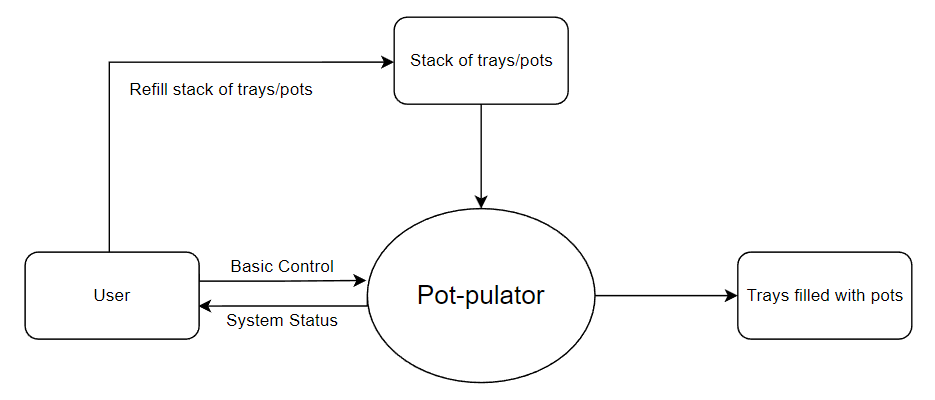
\includegraphics[width=\linewidth]{scope.PNG}
  \caption{System Context Diagram}
  \label{fig:scope}
\end{figure}

\section{Project Overview}

\subsection{Normal Behaviour}

The Pot-pulator needs to be filled with empty pots and trays by the user. Upon pressing the "start" button,
the Pot-pulator begins its operation with no further interaction required by the user.
Under normal operation, the ideal behaviour of the Pot-pulator will be as follows:
\begin{enumerate}
  \item User fills the machine with empty pots and trays
  \item User flips the power switch on
  \item User flips the conveyor switch on and the conveyor begins to move forward
  \item A tray will automatically drop down and begin moving along the conveyor
  \item The tray will hit 2 lever switches which lines up the tray to prepare for pot dispensing
  \item Stop the conveyor when pots are lined up with the next row on the tray and dispense 2 pots at a time in the tray
  \item Continue moving the conveyor to the next available pair of slots in the tray
  \item Repeat steps 6 and 7 until the entire tray is filled with pots (10 pots)
  \item Once the tray is filled with pots, the verification subsystem determines if all the pots have been placed correctly in the tray
\end{enumerate}

\noindent Throughout the opreation of the device, the user interface displays the current status of the machine.

\subsection{Undesired Event Handling}
The Pot-pulator is vulnerable to many undesired events during operation. The user will be notified should anything
go wrong with the system via the user interface, LEDs, and sound.
\subsubsection{Pot/Tray Misalignement}
A very common issue that could arise with the Pot-pulator is that there is the possibility
of a pot not being placed correctly in the tray due to misalignement. To mitigate this risk,
the verification subsystem was implemented to ensure that there are pots in all of the tray slots.
If there are missing pots, the user will be notified and the tray may be removed from the conveyor by hand.

\subsubsection{Motor Jam/Malfunction}
If a motor is unable to turn or fails, the system comes to a stop and the user is notfied about the issue.
The user is then expected to remove the object that is blocking the motor from moving. If the motor refuses to turn even without obstruction,
the motor will most likely need to be replaced by a qualified individual.


\subsection{Component Diagram}
\begin{figure}[H]
  \centering
  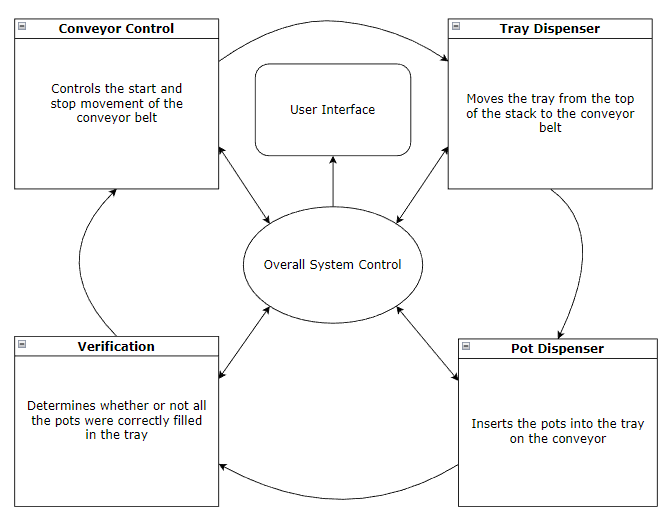
\includegraphics[width=\linewidth]{component_diagram.PNG}
  \caption{Component Diagram}
  \label{fig:componentdiagram}
\end{figure}
\subsection{Connection Between Requirements and Design} \label{SecConnection}

  The table below shows the traceability between design components and requirements specified in the SRS.
  
\begin{table}[H]
\caption{Requirements and System Design}
\begin{tabularx}{\textwidth}{|l|X|}
\hline
\textbf{Component} & \textbf{Corresponding Requirement} \\ \hline
Overall System Control  & NFR11, NFR12 \\ \hline
Conveyor Control   & CR1, CR2, CR3, CR4, CR5, CR6, NFR8 \\ \hline
Tray Dispenser   & TDR1, TDR2, TDR3, TDR4, TDR5, TDR6, TDR7, NFR4, NFR10, NFR13, NFR16 \\ \hline
Pot Dispenser   &  PDR1, PDR2, PDR3, PDR4, PDR5, PDR6, PDR7, PDR8, NFR4, NFR9, NFR14, NFR15  \\ \hline
Verification   &  VR1, VR2, NFR5 \\ \hline
User Interface  &  NFR7 \\ \hline
\end{tabularx}
\end{table}

\section{System Variables}


\subsection{Monitored Variables}
\begin{table}[H]
\caption{Monitored Variables}
\begin{tabular}{ |p{3cm}|p{9cm}|p{2cm}|p{1cm}| }
  \hline
  Variable & Description & Type & Units\\
  \hline
  Sensor Distances & Measured distances that the sensor identifies
   & Distance & mm\\
  \hline
  System State & Determines the state of the system (ie. Ready, Running, Error, Success)
   & State &  N/A\\
  \hline
  Tray/Pot Weight & Weight of the trays/pots to verify number in the stack
   & Weight & kg\\
  \hline
  Tray/Pot Height & Height of the trays/pots to verify number in the stack
   & Height & m\\
  
  \hline
 \end{tabular}\\\\
 \end{table}

\subsection{Controlled Variables}
\begin{table}[H]
\caption{Controlled Variables}
\begin{tabular}{ |p{3cm}|p{9cm}|p{2cm}|p{1cm}| }
  \hline
  Variable & Description & Type & Units\\
  \hline
  Motor Speeds & The speeds at which the motors in the system will turn
   & Speed & rad/s\\
  \hline
  Voltage In & Voltage going into the system
   & Voltage & V\\
  \hline
  Current In & Current going into the system
   & Current &  A\\
  \hline
  LEDs & LED status lights
   & Boolean & N/A\\
  
  \hline
 \end{tabular}\\\\
\end{table}

\subsection{Constants Variables}
\begin{table}[H]
  \caption{Constants Variables}
\begin{tabular}{ |p{3cm}|p{8.9cm}|p{2.1cm}|p{1cm}| }
  \hline
  Variable & Description & Type & Units\\
  \hline
  Motor Acceleration & The acceleration at which the motors in the system will turn
   & Acceleration & rad/s\textsuperscript{2}\\
  \hline
  Pots Dispensed & Pots dispensed by the system per cycle
   & Quantity & pots per cycle\\
  \hline
  Trays Dispensed & Trays dispensed by the system per cycle
   & Quantity &  trays per cycle\\
  \hline
  Total Distance & Total distance travelled by trays
   & Distance & m\\
  
  \hline
 \end{tabular}\\\\
\end{table}

\section{User Interfaces}


The User Interface will consist of a set of buttons to allow the operator to safely 
interact with the machine. It will also consist of audible and visual signals to alert
the operator of any action required (e.g. tray/pot restock, verification error, etc.).
See Appendix A for interface layout concept.

\section{Design of Hardware}

\subsection{Conveyor}

The conveyor subsystem will be comprised of:
\begin{itemize}
  \item 1 conveyor (including belt, motor, gear box and framing)
  \item 1 Arduino Uno microcontroller
  
\end{itemize}
The conveyor has been acquired from Sheridan Nurseries and will not require fabrication.


\subsection{Pot Dropper}

The pot dropper subsystem will be comprised of:
\begin{itemize}
  \item 1 Arduino Uno microcontroller
  \item 4 stepper motors (Nema-17)
  \item 4 stepper motor drivers (A4988)
  \item 4 custom pot dropper discs
  \item 1 ultrasonic range finder (HC-SR04)
  \item 2 lever switches
  \item screws and bracket mounts
  \item aluminum t-slotted extrusion
\end{itemize}
The pot dropper will be fabricated with steel x-beam framing to support the mechanism.
See Appendix B.1 for a CAD diagram of the pot dropper screw.

\subsection{Tray Dropper}

The tray dropper subsystem will be comprised of:
\begin{itemize}
  \item 1 Arduino Uno microcontroller
  \item 2 stepper motors (Nema-17)
  \item 2 stepper motor drivers (A4988)
  \item 2 custom tray dispenser gears
  \item 1 ultrasonic range finder (HC-SR04)
  \item 2 D-slotted steel shaft and connectors
  \item screws and bracket mounts
  \item aluminum T-slotted extrusion
\end{itemize}
The tray dropper will be fabricated with x-beam framing to support the mechanism. The 
stepper motors and belt bearings will be attached to the framing, and the belts will 
be secured to the bearings. See Appendix B.2 for a CAD diagram of the tray dropper 
end-effector.

\subsection{Conveyor Belt}

The conveyor belt used for the Pot-pulator is a 58 x 29.5 x 11.5 inch conveyor with a 50W AC motor driven by a custom printed
circuit board. Additional hardware components included:
\begin{itemize}
  \item 1 Arduino Uno microcontroller
  \item 2 ultrasonic range finders (HC-SR04)
  \item 1 mechanical relay (SDR-05VDC-SL-C)
\end{itemize}

\subsection{Verification}

The verification subsystem will be comprised of:
\begin{itemize}
  \item 2 ultrasonic range finders (HC-SR04)
\end{itemize}

\subsection{User Interface}

The user interface will be comprised of:
\begin{itemize}
  \item 1 Arduino Uno microcontroller
  \item 3.5 inch TFT 320x480 LCD (HXD8357D)
\end{itemize}

\section{Design of Electrical Components}

The Pot-pulator has a number of electrical components in the system. A complete overview of the circuit diagram
can be found in section C of the appendix. To improve modularity and for easier troubleshooting,
the electrical components were divided in to 4 subsystems based on the control of the system: conveyor control/verification, pot
dispensing, tray dispensing, and user interface. These subsystems are each controlled using an 
Arduino Uno while communicating with each other when necessary. For each subsystem,
its respective Arduino reads inputs from electronic components such as sensors, switches, and buttons and 
outputs control accordingly to the various motors. The Arduinos from each of the 
subsystems send a status bit to the LCD subsystem. If an error were to occur in
one of the subsystems, the LCD will show the appropriate status message and the entire system will act accordingly.



% \section{Design of Communication Protocols}

% \wss{If appropriate}

\section{Timeline}


\begin{table}[H]
  \caption{Timeline}
\begin{tabular}{ |p{3cm}|p{5cm}|p{4cm}|p{2cm}| }
  \hline
  Task & Description & Team Member(s) & Deadline\\
  \hline
  Pot Dropper Design & Design of pot dropper hardware and software
  & Juan Moncada and Gillian Ford & Juanuary 23, 2023\\
  \hline
  Tray Dropper Design & Design of tray dropper hardware and software
  & Steven Ramundi and Aaron Billones & January 23, 2023\\
  \hline
  Pot Dropper Fabrication & Fabrication of pot dropper frame and apparatus
  & Juan Moncada & January 31, 2023\\
  \hline
  Tray Dropper Fabrication & Fabrication of tray dropper and elevator frame and apparatus
  & Steven Ramundi and Aaron Billones & January 31, 2023\\
  \hline
  Verification Fabrication & Fabrication of verification System
  & Gillian Ford & January 31, 2023\\
  \hline
  Electrical Fabrication & Fabrication and assembly of all electrical components
  & All members & February 2, 2023\\
  \hline
  Testing & Testing of all subsystems and components
  & All members & February 6, 2023\\
  \hline

\end{tabular}
\end{table}

% \bibliographystyle {plainnat}
% \bibliography{../../../refs/References}

\newpage{}

\appendix

\section{Interface}

% \wss{Include additional information related to the appearance of, and
% interaction with, the user interface}
\begin{figure}[H]
  \centering
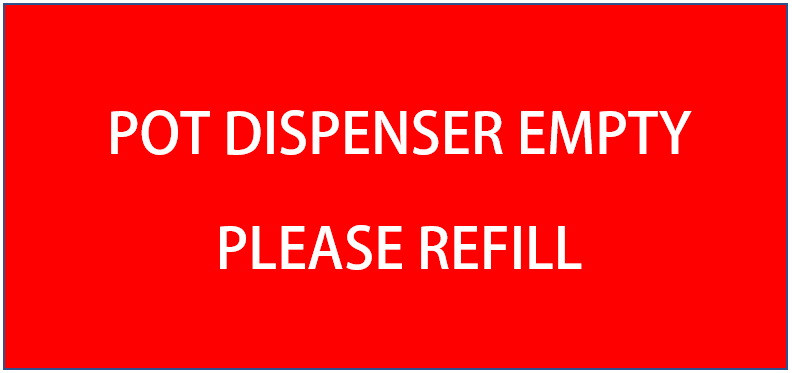
\includegraphics{interface1.png}
\caption{Example of Interface}
  \label{fig:interface1}
\end{figure}
The above figure shows an example of a status message alerting the machine operator that the pot 
dispenser requires refill. This would be accompanied by an audible alert.

\begin{figure}[H]
  \centering
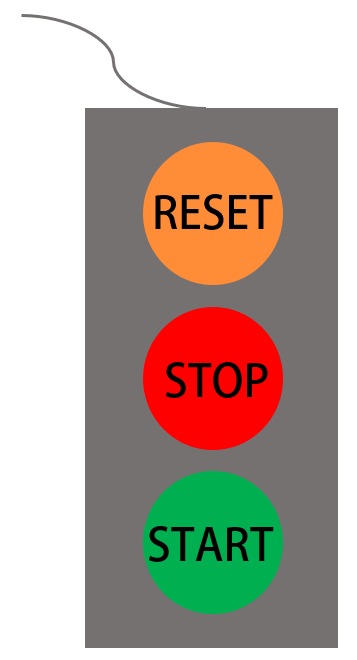
\includegraphics[width=0.25\textwidth]{interface2.png}
\caption{Example of Button Controls}
  \label{fig:interface2}
\end{figure}
Concept of the button interface used by the operator to control the machine. 
Handheld as to mitigate any safety concerns with a machine-mounted apparatus.

\section{Mechanical Hardware}

\subsection{Pot Dropper}
\begin{figure}[H]
  \centering
  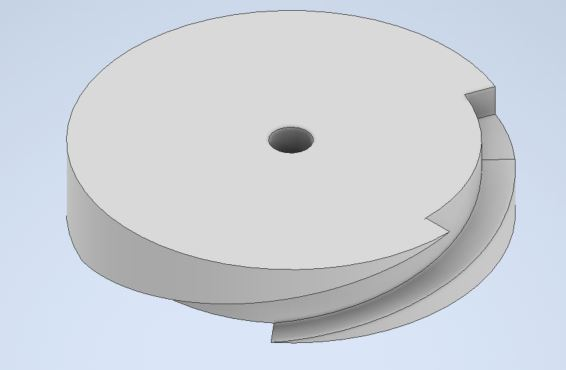
\includegraphics{Pot_Dropper.jpg}
  \caption{Tray Dropper End-Effector}
  \label{fig:potdropper1}
\end{figure}

\subsection{Tray Dropper}
\begin{figure}[H]
  \centering
  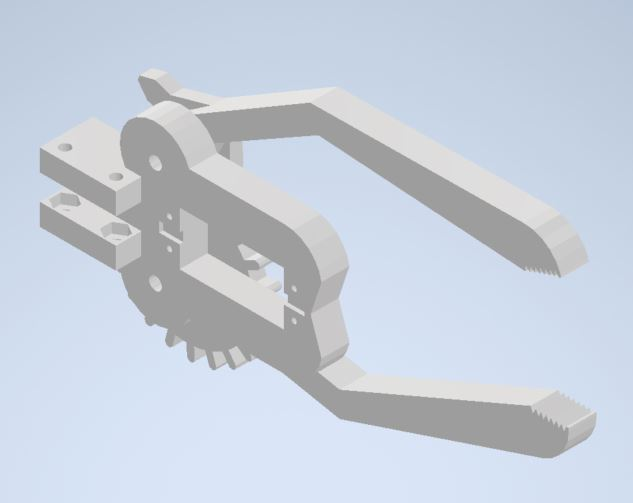
\includegraphics{Tray_Dropper.jpg}
  \caption{Tray Dropper End-Effector}
  \label{fig:traydropper1}
\end{figure}

\subsection{Tray Elevator}
\begin{figure}[H]
  \centering
  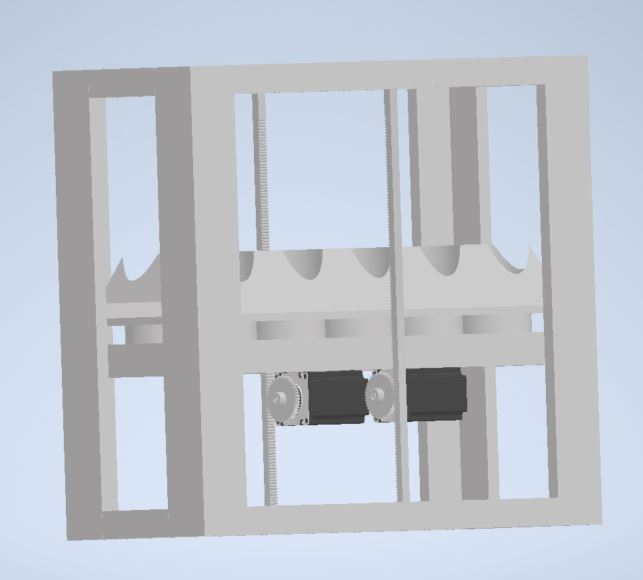
\includegraphics{Tray_Elevator.jpg}
  \caption{Tray Elevator (side)}
  \label{fig:elevator1}
\end{figure}

\begin{figure}[H]
  \centering
  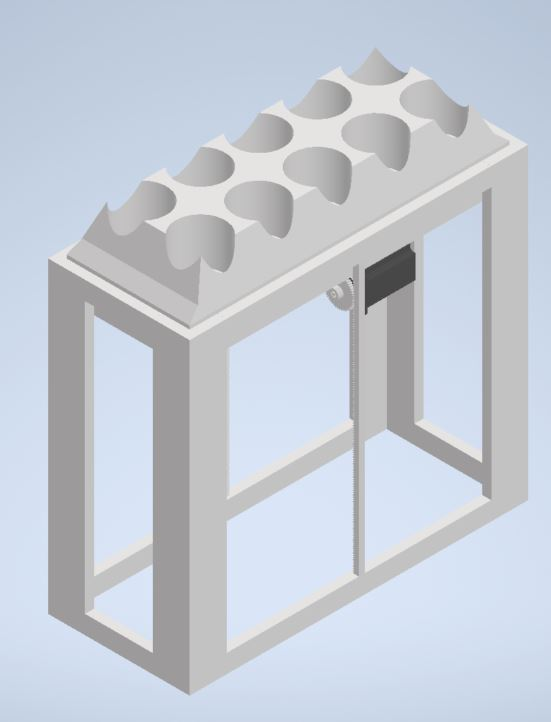
\includegraphics{Tray_Elevator2.jpg}
  \caption{Tray Elevator (orthographic projection)}
  \label{fig:elevator2}
\end{figure}

\section{Electrical Components}

\begin{figure}[H]
  \centering
  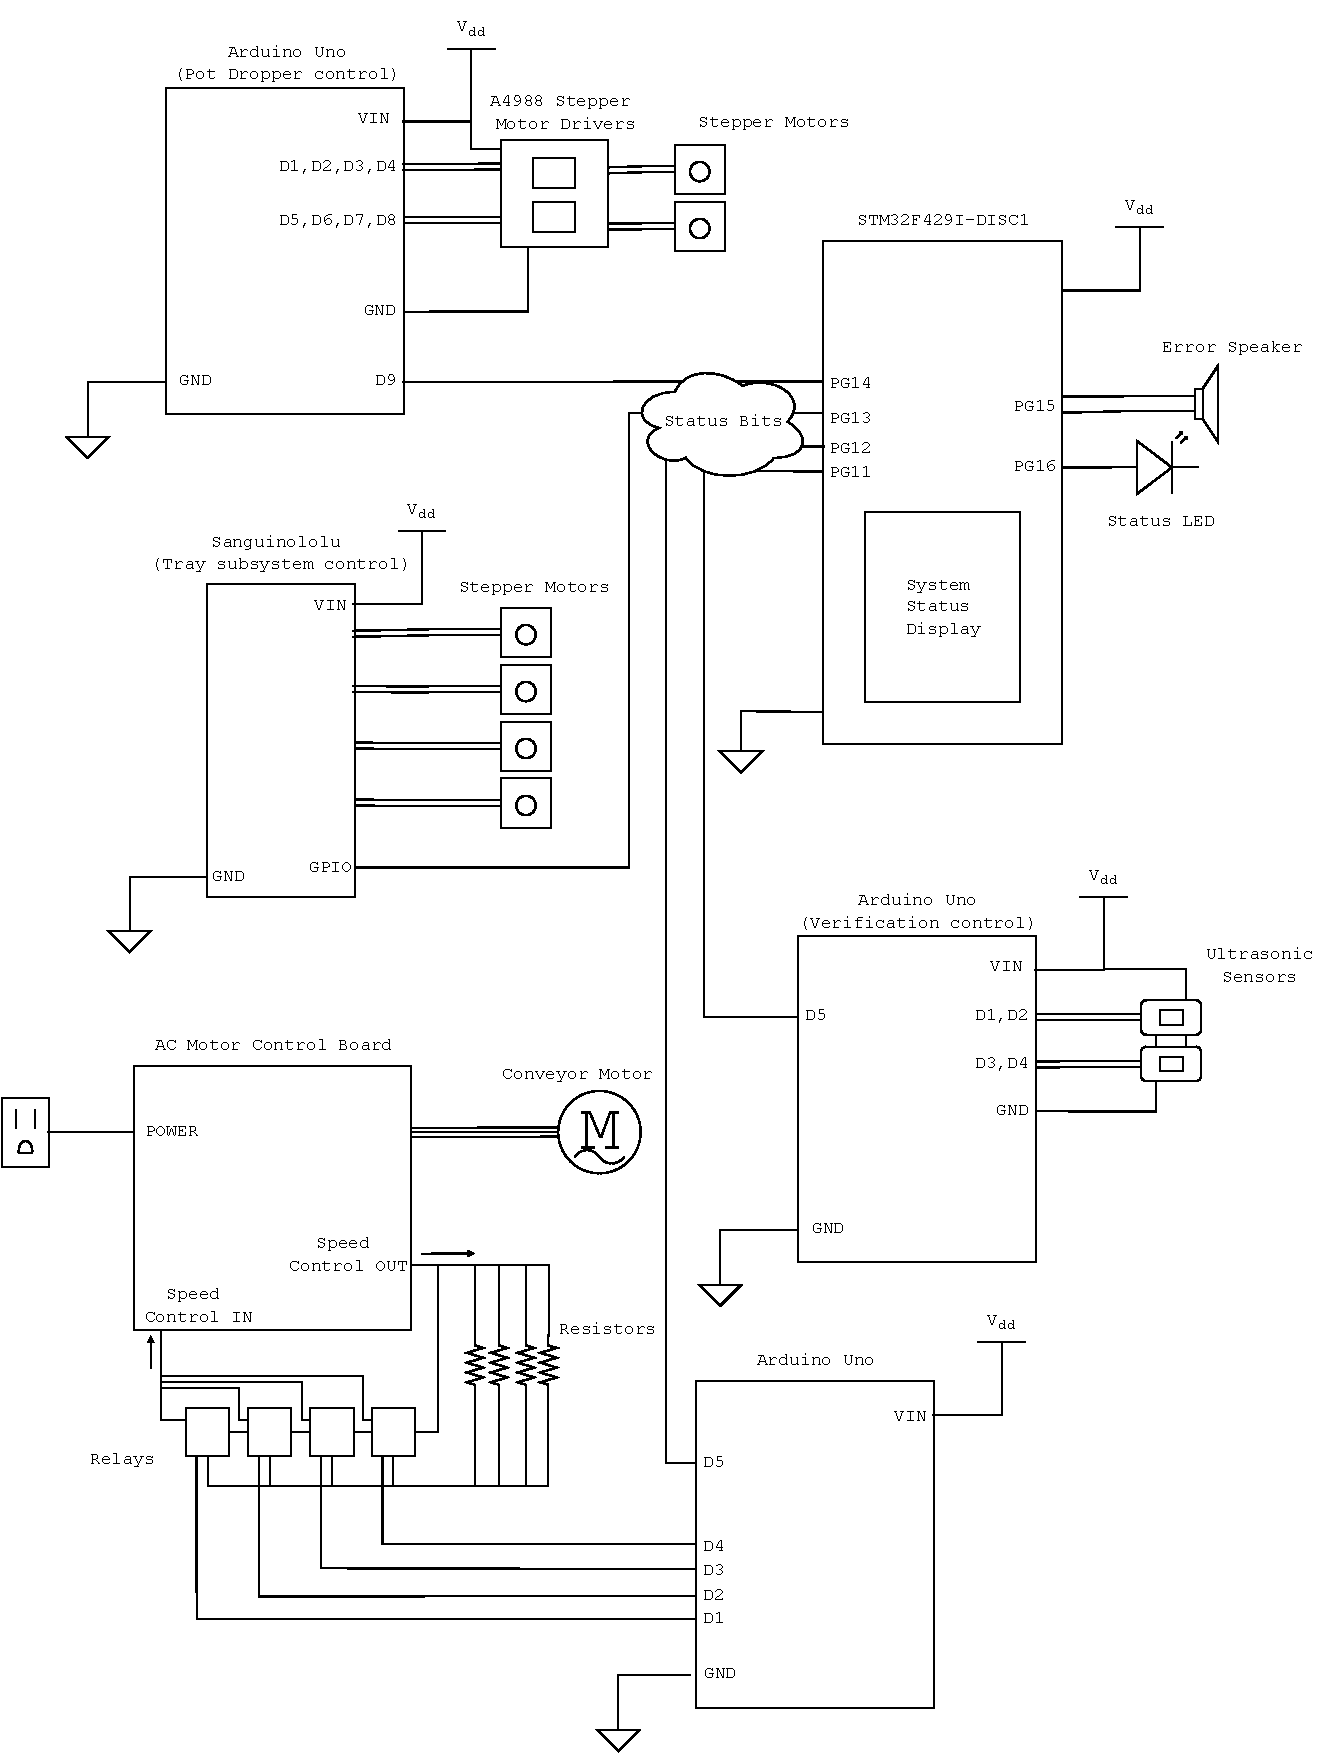
\includegraphics[width=0.89\textwidth]{circuit_diagram.pdf}
  \caption{Circuit Diagram}
  \label{fig:circuit}
\end{figure}


\section{Reflection}

The information in this section will be used to evaluate the team members on the
graduate attribute of Problem Analysis and Design.  Please answer the following questions:

\begin{enumerate}
  \item What are the limitations of your solution?  Put another way, given
  unlimited resources, what could you do to make the project better?\\

  One limitation of our solution would be the overall load capacity of the system.
  We are constrained by the space where the pots and trays are being stored in the device
  that makes it difficult to upsize. Another limitation of our solution is that there are only
  a set number of speeds we can make the conveyor move at relative to the number of relays we use.
  This is because we used the existing AC motor that came with the conveyor and its control board rather than
  designing a control board from scratch. We still wanted to control the AC motor with an Arduino in some way with digital signals.
  This created some issues in controlling the motor to an exact speed we wanted. Given unlimited resources,
  we would ideally get a conveyor system that had a DC motor and could seemlessly be controlled using 
  digital signals. We would also create more robust mounts and obtain more accurate sensors in order to mitigate risks
  during operation.
  

  \item Give a brief overview of other design solutions you considered.  What
  are the benefits and tradeoffs of those other designs compared with the chosen
  design?  From all the potential options, why did you select documented design?\\
  
  We considered a number of design solutions on each subsystem of our device. For controlling the AC motor (conveyor),
  we considered purchasing a digital potentiometer. This option would give us more precise control over the motor, 
  but was much more expensive that using relays. Another design option we considered was using a pully system to lift the 
  trays into position in preparation for dispensing. We opted out of this option because the pully system would be less accurate and reliable
  than our rack and pinion design. We considered dispensing the trays in a simiar way to the pots using a threaded dropping system. However,
  given the shape and flexibility of the trays, we determined that this would be a unreliable way of getting the trays on the conveyor. The 
  gantry method of moving the tray is much more reliable.
\end{enumerate}

\end{document}